%%
%% Start Definitions (each of these we can reuse)
%%
\begin{SaveDefinition}[
		key=SubsetSuperset,
		title={Subset \& Superset}
	]
	The set $B$ is a \emph{subset} of the set $A$, written $B\subseteq A$, if for all
	$b\in B$ we also have $b\in A$.  In this case, $A$ is called a \emph{superset}
	of $B$.\footnote{
		Some mathematicians use the symbol $\subset$ instead of $\subseteq$.}
\end{SaveDefinition}
\begin{SaveDefinition}[
		key=SetEquality,
		title={Set Equality}
	]
	The sets $A$ and $B$ are \emph{equal}, written $A=B$, if $A\subseteq B$ and $B\subseteq A$.
\end{SaveDefinition}
\begin{SaveDefinition}[
		key=SetSubtraction,
		title={Set Subtraction}
	]
	For sets $A$ and $B$, the \emph{set-wise difference}\index{set subtraction} between $A$ and $B$,
	written $A\backslash B$, is the set
	\[
		A\backslash B = \Set{x\given x\in A\text{ and }x\notin B}.
	\]
\end{SaveDefinition}
\begin{SaveDefinition}[
		key=UnionsIntersections,
		title={Unions \& Intersections}
	]
	Two common set operations are \emph{unions} and \emph{intersections}.
	Let $X$ and $Y$ be sets.

	\hfill\begin{minipage}{\dimexpr\textwidth-3cm}
	\begin{itemize}
		\item[(union)] $X\cup Y = \Set{ a \given a\in X\text{ or }a\in Y}$.
		\item[(intersection)] $X\cap Y = \Set{ a \given a\in X\text{ and }a\in Y}$.
	\end{itemize}
	\end{minipage}
\end{SaveDefinition}

\begin{SaveDefinition}[key=Set, title={Set}]
	A \emph{set} is a (possibly infinite) collection of items and is notated
	with curly braces (for example, $\{1,2,3\}$ is the set containing the
	numbers 1, 2, and 3). We call the items in a set
	\emph{elements}.

	If $X$ is a set and $a$ is an element of $X$, we may write $a\in X$,
	which is read ``$a$ is an element of $X$.''

	If $X$ is a set, a
	\emph{subset} $Y$ of $X$ (written $Y\subseteq X$) is a set such that
	every element of $Y$ is an element of $X$. Two sets are called
	\emph{equal} if they are subsets of each other (i.e., $X=Y$ if $X\subseteq
	Y$ and $Y\subseteq X$).

	We can define a subset using
	\emph{set-builder notation}. That is, if $X$ is a set, we can define the
	subset
	\[
		Y= \Set*{a\in X \given \text{some rule involving }a},
	\]
	 which is read ``$Y$ is the set of $a$ in $X$ {\bf such that} some rule
	involving $a$ is true.'' If $X$ is intuitive, we may omit it and simply write
	$Y=\{a:\text{some rule involving }a\}$. You may equivalently use ``$|$''
	instead of ``$:$'', writing $Y=\{a\,|\,\text{some rule involving }a\}$.
\end{SaveDefinition}

\begin{SaveDefinition}[key=ZeroVector, title={Zero Vector}]
		The \emph{zero vector}\index{zero vector}, notated as $\vec 0$\index{$\vec 0$},
		is the vector with no magnitude.
\end{SaveDefinition}

\begin{SaveDefinition}[key=LinearCombination, title={Linear Combination}]
	A \emph{linear combination} of the vectors
	$\vec v_{1},\vec v_{2},\ldots,\vec v_{n}$ is a vector
	\[
		\vec w = \alpha_{1}\vec v_{1}+\alpha_{2}\vec v_{2}+\cdots+\alpha_{n}\vec
		v_{n}.
	\]
	 The scalars $\alpha_{1},\alpha_{2},\ldots,\alpha_{n}$ are called the
	\emph{coefficients} of the linear combination.
\end{SaveDefinition}

\begin{SaveDefinition}[
	key=NonnegativeConvexLinearCombinations,
	title={Non-negative \& Convex Linear Combinations}]

	Let
	$\vec w=\alpha_{1}\vec v_{1}+\alpha_{2}\vec v_{2}+\cdots+\alpha_{n}\vec
	v_{n}.$
	The vector $\vec w$ is called a 
	\emph{non-negative} linear combination of
	$\vec v_{1},\vec v_{2},\ldots,\vec v_{n}$ if
	\[\alpha_{1},\alpha_{2},\ldots,\alpha_{n}\geq 0.\]

	The vector $\vec w$ is called a 
	\emph{convex} linear combination of
	$\vec v_{1},\vec v_{2},\ldots,\vec v_{n}$
	if \[\alpha_{1},\alpha_{2},\ldots,\alpha_{n}\geq 0\qquad\text{and}\qquad
	\alpha_{1}+\alpha_{2}+\cdots+\alpha_{n}=1.\]
\end{SaveDefinition}

\begin{SaveDefinition}[key=VectorFormofaLine, title={Vector Form of a Line}]
	Let $\ell$ be a line and let $\vec d$ and $\vec p$ be vectors. If $\ell=\Set{\vec
	x\given \vec x= t\vec d+\vec p\text{ for some } t\in\R }$ we say the vector equation

	\[
		\vec x=t\vec d+\vec p
	\]
	 is $\ell$ expressed in
	\emph{vector form}. The vector $\vec d$ is called a
	\emph{direction vector} for $\ell$.
\end{SaveDefinition}

\begin{SaveDefinition}[key=VectorFormofaPlane, title={Vector Form of a Plane}]
	A plane $\mathcal P$ is written in
	\emph{vector form} if it is expressed as
	\[
		\vec x=t\vec d_{1} +s\vec d_{2}+\vec p
	\]
	 for some vectors $\vec d_{1}$ and $\vec d_{2}$ and point $\vec p$. That
	is,
	$\mathcal P = \{\vec x: \vec x= t\vec d_{1}+s\vec d_{2} +\vec p\text{ for
	some }t,s\in\R \}$. The vectors $\vec d_{1}$ and $\vec d_{2}$ are called
	\emph{direction vectors} for $\mathcal P$.
\end{SaveDefinition}

\begin{SaveDefinition}[key=Span, title={Span}]
	The
	\emph{span} of a set of vectors $V$ is the set of all linear
	combinations of vectors in $V$. That is,
	\[
		\Span V = \Set{\vec v \given \vec v=\alpha_1\vec v_1+\alpha_2\vec
		v_2 + \cdots +\alpha_n\vec v_n\text{ for some }\vec v_1,\vec v_2,\ldots,\vec
		v_n\in V \text{ and scalars }\alpha_1,\alpha_2,\ldots,\alpha_n}.
	\]

	Additionally, we define $\Span\Set{} = \Set{\vec 0}$.
\end{SaveDefinition}

\begin{SaveDefinition}[key=SetAddition, title={Set Addition}]
	If $A$ and $B$ are sets of vectors, then the
	\emph{set sum} of $A$ and $B$, denoted $A+B$, is
	\[
		A+B=\Set{\vec x \given \vec x=\vec a+\vec b\text{ for some }\vec
		a\in A\text{ and } \vec b\in B}.
	\]

\end{SaveDefinition}

\begin{SaveDefinition}[
	key=LinearlyDependentIndependentGeometric,
	title={Linearly Dependent \& Independent (Geometric)}]

	We say the vectors $\vec v_{1},\vec v_{2},\ldots,\vec v_{n}$ are
	\emph{linearly dependent} if for at least one $i$,
	\[
		\vec v_{i}\in\Span\Set{\vec v_1,\vec v_2,\ldots,\vec v_{i-1}, \vec
		v_{i+1},\ldots,\vec v_n}.
	\]
	 Otherwise, they are called
	\emph{linearly independent}.
\end{SaveDefinition}

\begin{SaveDefinition}[
	key=TrivialLinearCombination,
	title={Trivial Linear Combination}]

	The linear combination $\alpha_1\vec v_1+\cdots+\alpha_n\vec v_n$ is called
	\emph{trivial}\index{trivial linear combination}
	if $\alpha_1=\cdots=\alpha_n=0$. If at least one $\alpha_i\neq 0$,
	the linear combination is called \emph{non-trivial}.
\end{SaveDefinition}

\begin{SaveDefinition}[
	key=LinearlyDependentIndependentAlgebraic,
	title={Linearly Dependent \& Independent (Algebraic)}]

	The vectors $\vec v_{1},\vec v_{2},\ldots,\vec v_{n}$ are
	\emph{linearly dependent} if there is a non-trivial linear combination
	of $\vec v_{1},\ldots,\vec v_{n}$ that equals the zero vector.
\end{SaveDefinition}

\begin{SaveDefinition}[
	key=HomogeneousSystem,
	title={Homogeneous System}]

	A system of linear equations or a vector equation in the variables $\alpha_1$, \ldots, 
	$\alpha_n$ is called
	\emph{homogeneous} if it takes the form
	\[
		\alpha_1\vec v_1+\alpha_2\vec v_2+\cdots +\alpha_n\vec v_n=\vec 0,
	\]
	where the right side of the equation is $\vec 0$.
\end{SaveDefinition}


\begin{SaveDefinition}[key=Norm, title={Norm}]
	The
	\emph{norm} of a vector $\vec v=\matc{v_1\\\vdots\\v_n}$ is the length/magnitude
	of $\vec v$. It is written $\|\vec v\|$ and can be computed from the Pythagorean
	formula
	\[
		\|\vec v\|=\sqrt{v_1^2+\cdots +v_n^2}.
	\]

\end{SaveDefinition}

\begin{SaveDefinition}[key=DotProduct, title={Dot Product}]
	If $\vec a=\matc{a_1\\a_2\\ \vdots\\a_n}$ and
	$\vec b=\matc{b_1\\b_2\\ \vdots\\b_n}$ are two vectors in $n$-dimensional
	space, then the
	\emph{dot product} of $\vec a$ an $\vec b$ is
	\[
		\vec a\cdot\vec b = a_{1}b_{1}+a_{2}b_{2}+\cdots+a_{n}b_{n}.
	\]
	 Equivalently, the dot product is defined by the geometric formula
	\[
		\vec a\cdot \vec b = \|\vec a\|\|\vec b\|\cos \theta
	\]
	 where $\theta$ is the angle between $\vec a$ and $\vec b$.
\end{SaveDefinition}

\begin{SaveDefinition}[key=Direction, title={Direction}]
	The vector $\vec u$ points in the \emph{direction} of
	the vector $\vec v$ if $k\vec u=\vec v$ for some scalar $k$.
	The vector $\vec u$ points in the \emph{positive direction} of
	$\vec v$ if $k\vec u=\vec v$ for some positive scalar $k$.
\end{SaveDefinition}

\begin{SaveDefinition}[key=Distance, title={Distance}]
	The
	\emph{distance} between two vectors $\vec u$ and $\vec v$ is
	$\|\vec u-\vec v\|$.
\end{SaveDefinition}

\begin{SaveDefinition}[key=UnitVector, title={Unit Vector}]
	A vector $\vec v$ is called a
	\emph{unit vector} if $\|\vec v\|=1$.
\end{SaveDefinition}

\begin{SaveDefinition}[key=Orthogonal, title={Orthogonal}]
	Two vectors $\vec u$ and $\vec v$ are
	\emph{orthogonal} to each other if $\vec u\cdot \vec v=0$. The word orthogonal
	is synonymous with the word perpendicular.
\end{SaveDefinition}

\begin{SaveDefinition}[key=NormalVector, title={Normal Vector}]
	A
	\emph{normal vector} to a line (or plane or hyperplane) is a non-zero
	vector that is orthogonal to all direction vectors for the line (or plane
	or hyperplane).
\end{SaveDefinition}

\begin{SaveDefinition}[key=NormalFormofaLine, title={Normal Form of a Line}]
	A line $\ell\subseteq \R^2$ is expressed in \emph{normal form} if $\ell$
	is the solution set to the equation
	\[
		\vec n\cdot (\vec x-\vec p)=0
	\]
	where $\vec n$ and $\vec p$ are fixed vectors.
\end{SaveDefinition}

\begin{SaveDefinition}[key=Hyperplane, title={Hyperplane}]
	The set $X\subseteq \R^n$ is called a \emph{hyperplane} if there
	exists $\vec n\neq \vec 0$ and $\vec p$ so that $X$ is the set of solutions
	to the equation
	\[
		\vec n\cdot (\vec x-\vec p)=0.
	\]
\end{SaveDefinition}


\begin{SaveDefinition}[key=Projection, title={Projection}]
	Let $X$ be a set. The
	\emph{projection} of the vector $\vec v$ onto $X$, written $\Proj_{X}\vec
	v$, is the closest point in $X$ to $\vec v$.
\end{SaveDefinition}

\begin{SaveDefinition}[key=Component, title={Vector Components}]
	Let $\vec u$ and $\vec v\neq \vec 0$ be vectors. The
	\emph{vector component of $\vec u$ in the $\vec v$ direction}, written $\Comp_{\vec
	v}\vec u$, is the vector in the direction of $\vec v$ so that
	$\vec u-\Comp_{\vec v}\vec u$ is orthogonal to $\vec v$.
	\begin{center}
		\usetikzlibrary{patterns, decorations.pathreplacing}
		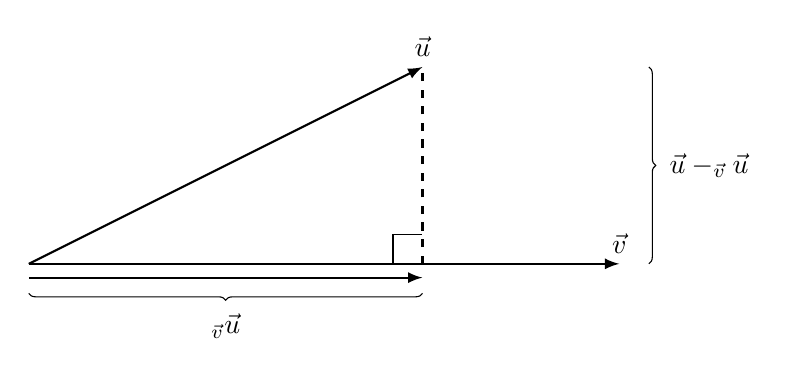
\begin{tikzpicture}[>=latex, scale=2.5]
			\draw[->,thick,black] (0,0) -- (2,1) node [above]
				{$\vec u$};

			\draw[->,thick,black] (0,0) -- (3,0) node [above]
				{$\vec v$};

			\draw[->,thick,black,yshift=-.07cm] (0,0) -- (2,0);
			\draw[decoration={brace, mirror}, decorate, yshift=-.15cm]
				(0,0) -- (2,0) node [midway,below,yshift=-4pt] {$\Comp_{\vec
				v}\vec u$};

			\draw[dashed,thick,black] (2,0) -- (2,1);
			\draw[decoration={brace, mirror}, decorate, xshift=1.15cm]
				(2,0) -- (2,1) node [midway,right,xshift=4pt]
				{$\vec u-\Comp_{\vec v}\vec u$};

			\draw[thin,black] (1.85,0)--(1.85,.15)--(2,.15);
		\end{tikzpicture}
	\end{center}
\end{SaveDefinition}

\begin{SaveDefinition}[key=Subspace, title={Subspace}]
	A non-empty subset $V\subseteq \R^{n}$ is called a \emph{subspace} if for all $\vec u,\vec v\in V$ and all
	scalars $k$ we have
	\begin{enumerate}
		\item[(i)] $\vec u+\vec v\in V$; and

		\item[(ii)] $k\vec u\in V$.
	\end{enumerate}
\end{SaveDefinition}

\begin{SaveDefinition}[key=TrivialSubspace, title={Trivial Subspace}]
	The subset $\Set{\vec 0}\subseteq\R^n$ is called the \emph{trivial subspace}.
\end{SaveDefinition}

\begin{SaveDefinition}[key=Basis, title={Basis}]
	A
	\emph{basis} for a subspace $\mathcal V$ is a linearly independent set of vectors,
	$\mathcal B$, so that $\Span\mathcal B=\mathcal V$.
\end{SaveDefinition}

\begin{SaveDefinition}[key=Dimension, title={Dimension}]
	The
	\emph{dimension} of a subspace $V$ is the number of elements in a basis
	for $V$.
\end{SaveDefinition}

\begin{SaveDefinition}[key=StandardBasisforRn, title={Standard Basis}]
	The \emph{standard basis} for $\R^n$ is the set $\Set{\vec e_1,\ldots,\vec e_n}$ where
	\[
		\vec e_1=\matc{1\\0\\0\\\vdots}\qquad
		\vec e_2=\matc{0\\1\\0\\\vdots}\qquad
		\vec e_3=\matc{0\\0\\1\\\vdots}\qquad\cdots.
	\]
	That is $\vec e_i$ is the vector with a $1$ in its
	$i$th coordinate and zeros elsewhere.
\end{SaveDefinition}

\begin{SaveDefinition}[
	key=RepresentationinaBasis,
	title={Representation in a Basis}]

	Let $\mathcal B=\Set{\vec b_1,\ldots,\vec b_n}$ be a basis for a
	subspace $V$ and let $\vec v\in V$. The
	\emph{representation of $\vec v$ in the $\mathcal B$ basis}, notated $[\vec
	v]_{\mathcal B}$, is the column matrix
	\[
		[\vec v]_{\mathcal B}= \matc{\alpha_1\\\vdots\\\alpha_n}
	\]
	 where $\alpha_{1},\ldots,\alpha_{n}$ uniquely satisfy
	$\vec v=\alpha_{1}\vec b_{1}+\cdots+\alpha_{n}\vec b_{n}.$

	Conversely,
	\[
		\matc{\alpha_1\\\vdots\\\alpha_n}_{\mathcal B}= \alpha_{1}\vec b_{1}+\cdots
		+\alpha_{n}\vec b_{n}
	\]
	 is notation for the linear combination of $\vec b_{1},\ldots,\vec b_{n}$
	with coefficients $\alpha_{1},\ldots,\alpha_{n}$.
\end{SaveDefinition}

\begin{SaveDefinition}[key=OrthonormalBasis, title={Orthonormal Basis}]
	A basis $\mathcal B=\{\vec b_{1},\ldots,\vec b_{n}\}$ is called
	\emph{orthonormal} if every basis vector is a unit vector and all
	basis vectors are orthogonal to each other. That is,
	\[
		\vec b_i\cdot \vec b_j=\begin{cases}
			1 &\text{ if }\quad i=j\\
			0 &\text{ if }\quad i\neq j
		\end{cases}.
	\]
\end{SaveDefinition}

\begin{SaveDefinition}[key=OrientationofaBasis, title={Orientation of a Basis}]
	The ordered basis $\mathcal B=\{\vec b_{1},\ldots,\vec b_{n}\}$ is
	\emph{right-handed} or
	\emph{positively oriented} if it can be continuously transformed to the
	standard basis (with $\vec b_{i}\mapsto \vec e_{i}$) while remaining
	linearly independent throughout the transformation. Otherwise,
	$\mathcal B$ is called
	\emph{left-handed} or
	\emph{negatively oriented}.
\end{SaveDefinition}

\begin{SaveDefinition}[key=LinearTransformation, title={Linear Transformation}]
	Let $V$ and $W$ be subspaces. A function $T:V\to W$ is called a
	\emph{linear transformation} if
	\[
		T(\vec u+\vec v)=T\vec u+T\vec v \qquad\text{and}\qquad T(\alpha
		\vec v)=\alpha T\vec v
	\]
	 for all vectors $\vec u,\vec v\in V$ and all scalars $\alpha$.
\end{SaveDefinition}

\begin{SaveDefinition}[key=ImageofaSet, title={Image of a Set}]
	Let $L:\R^n\to \R^m$ be a transformation and let $X\subseteq \R^n$ be a set. The
	\emph{image of the set $X$ under $L$}, denoted $L(X)$, is the set
	\[
		L(X)=\Set{\vec x\in W \given \vec x=L(\vec y)\text{ for some }\vec
		y\in X}.
	\]

\end{SaveDefinition}

\begin{SaveDefinition}[key=CompositionofFunctions, title={Composition of Functions}]
	Let $f:A\to B$ and $g:B\to C$. The \emph{composition} of $g$ and $f$, notated $g\circ f$,
	is the function $h:A\to C$ defined by
	\[
		h(x)=g\circ f(x) = g\Big(f(x)\Big).
	\]
\end{SaveDefinition}

\begin{SaveDefinition}[key=Range, title={Range}]
	The
	\emph{range} (or
	\emph{image}) of a linear transformation $T:V\to W$ is the set of vectors
	that $T$ can output. That is,
	\[
		\Range(T)=\Set{\vec y\in W \given \vec y=T\vec x\text{ for some }\vec
		x\in V}.
	\]

\end{SaveDefinition}

\begin{SaveDefinition}[key=NullSpace, title={Null Space}]
	The
	\emph{null space} (or
	\emph{kernel}) of a linear transformation $T:V\to W$ is the set of vectors
	that get mapped to zero under $T$. That is,
	\[
		\Null(T)=\Set{\vec x\in V \given T\vec x=\vec 0}.
	\]

\end{SaveDefinition}

\begin{SaveDefinition}[
	key=InducedTransformation,
	title={Induced Transformation}]

	Let $M$ be an $n\times m$ matrix. We say $M$
	\emph{induces} a linear transformation $\mathcal T_{M}:\R^{m}\to\R^{n}$ defined
	by
	\[
		[\mathcal T_{M}\vec v]_{\mathcal E'}= M[\vec v]_{\mathcal E},
	\]
	 where $\mathcal E$ is the standard basis for $\R^{m}$ and $\mathcal E'$
	is the standard basis for $\R^{n}$.
\end{SaveDefinition}

\begin{SaveDefinition}[
	key=Transpose,
	title={Transpose}]

	Let $M$ be an $n\times m$ matrix defined by
	\[
		M=\matc{
			a_{11}&a_{12}&a_{13}&\cdots & a_{1m}\\
		a_{21}&a_{22}&a_{23}&\cdots&a_{2m}\\
		\vdots &\vdots&\vdots &\ddots&\vdots\\
		a_{n1}&a_{n2}&a_{3n}&\cdots&a_{nm}}.
	\]
	The \emph{transpose} of $M$, notated $M^T$ is the $m\times n$ matrix $M$ with its rows and
	columns swapped. That is
	\[
		M^T=\matc{
		a_{11}&a_{21}&\cdots&a_{m1}\\
		a_{12}&a_{22}&\cdots&a_{m2}\\
		a_{13}&a_{23}&\cdots&a_{m3}\\
		\vdots&\vdots&\ddots&\vdots\\
		a_{1n}&a_{2n}&\cdots&a_{mn}}.
	\]
\end{SaveDefinition}

\begin{SaveDefinition}[
	key=ElementaryMatrix,
	title={Elementary Matrix}]

	A matrix is called an \emph{elementary matrix} if it is an identity matrix with a single elementary row operation applied.
\end{SaveDefinition}

\begin{SaveDefinition}[
	key=MatrixInverse,
	title={Matrix Inverse}]
		
	The \emph{inverse} of a matrix $A$ is a
		matrix $B$ such that $AB=I$ and $BA=I$.
		In this case, $B$ is called the inverse of $A$ and is notated by $A^{-1}$.
\end{SaveDefinition}

\begin{SaveDefinition}[
	key=IdentityFunction,
	title={Identity Function}]
	
	Let $X$ be a set. The \emph{identity function} with domain and codomain $X$,
	notated $\Ident:X\to X$, is the function satisfying
	\[
		\Ident(x)=x
	\]
	for all $x\in X$.
\end{SaveDefinition}

\begin{SaveDefinition}[
	key=InverseFunction,
	title={Inverse Function}]
		
	Let $f:X\to Y$ be a function. We say $f$ is \emph{invertible} if
	there exists a function $g:Y\to X$ so that $f\circ g=\Ident$ and $g\circ f=\Ident$.
	In this case, we call $g$ an \emph{inverse} of $f$ and write
	\[
		f^{-1}=g.
	\]
\end{SaveDefinition}

\begin{SaveDefinition}[
	key=Onetoone,
	title={One-to-one}]
		
	Let $f:X\to Y$ be a function. We say $f$ is \emph{one-to-one} (or \emph{surjective}) if
	distinct inputs to $f$ produce distinct outputs. That is $f(x)=f(y)$ implies $x=y$.
\end{SaveDefinition}

\begin{SaveDefinition}[
	key=Onto,
	title={Onto}]
		
	Let $f:X\to Y$ be a function.
	We say $f$ is \emph{onto} (or \emph{injective}) if every point in the codomain of $f$ gets mapped to.
	That is $\Range(f)=Y$.
\end{SaveDefinition}

\begin{SaveDefinition}[
	key=IdentityMatrix,
	title={Identity Matrix}]
	
	An \emph{identity matrix} is a square matrix with ones on the diagonal
	and zeros everywhere else. The $n\times n$ identity matrix is denoted $I_{n\times n}$,
	or just $I$ when its size is implied.
\end{SaveDefinition}

\begin{SaveDefinition}[key=FundamentalSubspaces, title={Fundamental Subspaces}]
	Associated with any matrix $M$ are three fundamental subspaces: the
	\emph{row space} of $M$, denoted $\Row(M)$, is the span of the rows of
	$M$; the
	\emph{column space} of $M$, denoted $\Col(M)$, is the span of the
	columns of $M$; and the
	\emph{null space} of $M$, denoted $\Null(M)$, is the set of solutions to
	$M\vec x=\vec 0$.
\end{SaveDefinition}

\begin{SaveDefinition}[key=RankofaLinearTransformation, title={Rank of a Linear Transformation}]
	For a linear transformation $T:\R^n\to \R^m$, the
	\emph{rank} of $T$, denoted $\Rank(T)$, is the dimension of the range of
	$T$.
\end{SaveDefinition}

\begin{SaveDefinition}[key=RankofaMatrix, title={Rank of a Matrix}]
	Let $M$ be a matrix.
	The \emph{rank} of $M$, denoted $\Rank(M)$, is the rank of
	the linear transformation induced by $M$.
\end{SaveDefinition}

\begin{SaveDefinition}[key=NullityofaMatrix, title={Nullity of a Matrix}]
	Let $M$ be a matrix.
	The \emph{nullity} of $M$, denoted $\Rank(M)$, is the nullity of
	the linear transformation induced by $M$.
\end{SaveDefinition}

\begin{SaveDefinition}[key=Rank, title={Rank}]
	For a linear transformation $T:\R^n\to \R^m$, the
	\emph{rank} of $T$, denoted $\Rank(T)$, is the dimension of the range of
	$T$.

	For an $n\times m$ matrix $M$, the
	\emph{rank} of $M$, denoted $\Rank(M)$, is the number of pivots in
	$\rref(M)$.
\end{SaveDefinition}

\begin{SaveDefinition}[key=Nullity, title={Nullity}]
	For a linear transformation $T:\R^n\to \R^m$, the
	\emph{nullity} of $T$, denoted $\Nullity(T)$, is the dimension of the null space of
	$T$.
\end{SaveDefinition}

\begin{SaveDefinition}[key=ChangeofBasisMatrix, title={Change of Basis Matrix}]
	Let $\mathcal A$ and $\mathcal B$ be bases for $\R^n$. The matrix $M$ is called
	a \emph{change of basis} matrix converting from $\mathcal A$ to $\mathcal B$ if
	\[
		M[\vec x]_{\mathcal A}=[\vec x]_{\mathcal B}
	\]
	for all $\vec x\in \R^n$. Notationally, $\BasisChange{\mathcal A}{\mathcal B}$
	stands for the change of basis matrix converting from $\mathcal A$ to $\mathcal B$,
	and we may write $M=\BasisChange{\mathcal A}{\mathcal B}$.
\end{SaveDefinition}

\begin{SaveDefinition}[key=LinearTransformationinaBasis, title={Linear Transformation in a Basis}]
	Let $\mathcal T:\R^n\to\R^n$ be a linear transformation and let $\mathcal B$ be a
	basis for $\R^n$. The \emph{matrix for $\mathcal T$ with respect to $\mathcal B$}, notated
	$[\mathcal T]_{\mathcal B}$,
	is the $n\times n$ matrix satisfying
	\[
		[\mathcal T\vec x]_{\mathcal B} = [\mathcal T]_{\mathcal B}[\vec x]_{\mathcal B}.
	\]
	In this case, we say the matrix $[\mathcal T]_{\mathcal B}$ is the representation
	of $\mathcal T$ in the $\mathcal B$ basis.
\end{SaveDefinition}

\begin{SaveDefinition}[key=SimilarMatrices, title={Similar Matrices}]
	The matrices $A$ and $B$ are called
	\emph{similar matrices}, denoted $A\sim B$, if $A$ and $B$ represent the
	same linear transformation but in possibly different bases. Equivalently,
	$A\sim B$ if there is an invertible matrix $X$ so that
	\[
		A=XBX^{-1}.
	\]

\end{SaveDefinition}

\begin{SaveDefinition}[key=Unitncube, title={Unit $n$-cube}]
	The
	\emph{unit $n$-cube} is the $n$-dimensional cube with sides given by the
	standard basis vectors and lower-left corner located at the origin. That
	is
	\[
		C_{n}=\Set*{\vec x\in\R^n:\vec x=\sum_{i=1}^n\alpha_i\vec e_i\text{
		for some }\alpha_1,\ldots,\alpha_n\in[0,1]}=[0,1]^{n}.
	\]

\end{SaveDefinition}

\begin{SaveDefinition}[key=Determinant, title={Determinant}]
	The
	\emph{determinant} of a linear transformation $X:\R^{n}\to \R^{n}$, denoted $\det(X)$ or $\Abs{X}$, is
	the oriented volume of the image of the unit $n$-cube. The determinant of
	a square matrix is the determinant of its induced transformation.
\end{SaveDefinition}

\begin{SaveDefinition}[key=OrientationPreservingLinearTransformation, title={Orientation Preserving Linear Transformation}]
	Let $\mathcal T:\R^n\to\R^n$ be a linear transformation. We say $\mathcal T$
	is \emph{orientation preserving} if the ordered basis $\Set{\mathcal T(\vec e_1),\ldots, \mathcal T(\vec e)}$
	is a positively oriented  and we say $\mathcal T$
	is \emph{orientation reversing} if the ordered basis $\Set{\mathcal T(\vec e_1),\ldots, \mathcal T(\vec e)}$
	is a negatively. If $\Set{\mathcal T(\vec e_1),\ldots, \mathcal T(\vec e)}$
	is not a basis for $\R^n$, then $\mathcal T$ is neither orientation preserving nor orientation reversing.
\end{SaveDefinition}

\begin{SaveDefinition}[key=Eigenvector, title={Eigenvector}]
	Let $X$ be a linear transformation or a matrix. An
	\emph{eigenvector} for $X$ is a non-zero vector that doesn't change
	directions when $X$ is applied. That is, $\vec v\neq \vec 0$ is an
	eigenvector for $X$ if
	\[
		X\vec v=\lambda \vec v
	\]
	 for some scalar $\lambda$. We call $\lambda$ the
	\emph{eigenvalue} of $X$ corresponding to the eigenvector $\vec v$.
\end{SaveDefinition}

\begin{SaveDefinition}[
	key=CharacteristicPolynomial,
	title={Characteristic Polynomial}]

	For a matrix $A$, the
	\emph{characteristic polynomial} of $A$ is
	\[
		\chr(A)=\det(A-\lambda I).
	\]

\end{SaveDefinition}

\begin{SaveDefinition}[key=Diagonalizable, title={Diagonalizable}]
	A matrix is
	\emph{diagonalizable} if it is similar to a diagonal matrix.
\end{SaveDefinition}

\begin{SaveDefinition}[key=Eigenspace, title={Eigenspace}]
	Let $A$ be an $n\times n$ matrix with eigenvalues
	$\lambda_{1},\ldots,\lambda_{m}$. The
	\emph{eigenspace} of $A$ corresponding to the eigenvalue $\lambda_{i}$
	is the null space of $A-\lambda_{i} I$. That is, it is the space spanned
	by all eigenvectors that have the eigenvalue $\lambda_{i}$.

	The
	\emph{geometric multiplicity} of an eigenvalue $\lambda_{i}$ is the
	dimension of the corresponding eigenspace. The
	\emph{algebraic multiplicity} of $\lambda_{i}$ is the number of times
	$\lambda_{i}$ occurs as a root of the characteristic polynomial of $A$ (i.e.,
	the number of times $x-\lambda_{i}$ occurs as a factor).
\end{SaveDefinition}


